\documentclass[12pt]{article}

\usepackage{geometry}
%\geometry{margin=1in}

\usepackage{setspace}
\doublespacing

\usepackage{graphicx}

\usepackage[utf8]{inputenc}

% for \url{}
\usepackage{hyperref}

\title{Compute Servers for Teaching Big Data}
\author{Clark Fitzgerald}
\begin{document}

\maketitle

\begin{abstract}

% 112 words in abstract
% 4500 words in document
    We compare and contrast different compute server options for teaching an undergraduate statistics class centered on analyzing large, real world data sets located on powerful remote servers.
These options include institutionally supported servers, personal physical servers, public cloud services, and commercial cloud services.
% TODO: Align these options with the sections
We briefly describe the course, share our experience with each of these options including advantages and disadvantages, mention some technical considerations, and suggest when to choose which option.
Looking to the future, we outline requirements for a broadly shared educational compute service that will allow more instructors to teach similar classes without the overhead of having to manage and administer their own server.

\emph{keywords: big data, cloud computing, data science, teaching}

\end{abstract}

% TODO: Context, definitions, goals of the course, benefits of such a course to students


\section{The Course}

Stat 129, `Analyzing and Processing Big Data', is an upper division elective course offered by the Mathematics and Statistics Department at CSU Sacramento, and is required for students pursuing a bachelor's degree in Statistics with an Emphasis in Data Science.
The catalog course description is:

\emph{
Statistical analysis of large, complex data sets. Topics include memory efficient data processing, the split-apply-combine strategy, rewriting programs for scalability, handling complex data formats, and applications such as statistical learning, dimension reduction, and efficient data representation. Students will access data and run code on remote servers.
}

Stat 129 uses technologies including bash, Python, and SQL to analyze large data sets, with the intention of exposing students to the common tools in data science.
Students tend to be highly motivated, because many of them hope to land jobs requiring these skills after graduation.
Stat 129 requires a programming prerequisite, since it is too advanced for a first programming course.
Statistics majors take Stat 129 after taking `Statistical Computing', an upper division course focused on data analysis using the R programming language, with content similar to Data Science in a Box, R4DS TODO: Cite.
%Ideally, students would have taken two semesters of programming before this course.

The philosophy behind this class is to provide students with real world data sets and ask open ended questions, following in the footsteps of our teachers and mentors, Deborah Nolan and Duncan Temple Lang \cite{nolan2010computing}.
We have been teaching data science programming technologies in an academic setting since 2015, and we developed Stat 129 and have taught it each year since 2021.
Feedback from this data forward approach in general, and this class in particular, has been overwhelmingly positive.
In Stat 129 students ask real questions based on real data that resides on a real server, and for this reason several alumni have reported that this has been the single most practical and valuable class that they have taken in college.

\subsection{Which Data?}
\label{sec:data}

%The term `Big Data' appears in the title for Stat 129; for this term to be more than a buzz word, we need to define it.
% TODO: Could talk about how others use this term.
For the purposes of Stat 129, `big data' means a data set that is large enough such that one cannot load the entire data set into a laptop's memory at once.
In a typical introductory data analysis class, a student reads a single data file into R or Python and proceeds with the analysis steps \cite{dsbox}.
This works great if the data fits into memory, but if the data does not fit into memory, then it simply doesn't work.
Data sets that are larger than memory require entirely different approaches, such as streaming through to filter out a subset of interest.
%Once a data set is this large, it's not possible to simply load the whole thing and start working using R or Python.
Our goal is to choose data sets that are comfortably over this memory threshold, such that the techniques we're learning are motivated, but not gratuitously large such that answering a basic question takes an excessive amount of time.
Practically speaking, at the time of this writing, a typical student laptop will have between 4 and 32 GB of memory, and data sets that are on the order of 10-100 GB on disk work well to motivate the techniques.
We assign common data analysis tasks that typically take 1 to 10 minutes if done in serial, and are an order of magnitude faster if done in parallel.

%While teaching this course, we have to select data sets.
%Everything that we do in the course is based on working with a legitimate, unwieldy, data set.
When teaching Stat 129, we look for data sets that satisfy the criteria below.
\begin{enumerate}
\item \textbf{Size} The files should be large enough to motivate the computational techniques we're learning, but no larger, as described above.
\item \textbf{Publicly Available} The data should be readily available for legal public download.
	Special permissions, non disclosure agreements, and licensing all take time away from teaching.
\item \textbf{Format} The storage format should be a common one that students will encounter in data science work, so that students can directly apply what they learn in class.
	Avoid proprietary, novel, or highly specialized data formats.
    Each semester of Stat 129, we work with data in a plain text tabular format such as CSV or TSV, and nested formats such as XML or JSON.
\item \textbf{Background Knowledge} A college student should be able to understand what the data actually represents.
	If it takes longer than a single class period to explain the core idea of what the data captures, then that data is probably too complex.
\end{enumerate}
These criteria don't necessarily apply to more domain specific classes, for example, a bioinformatics class studying genomes would do well to focus on genomic data.
%Most of these principles We've violated at one time or another, and the difficulties became clear later.
Amazon Open Data\footnote{\url{https://registry.opendata.aws/}} has provided a reliably good source of large data sets fitting these criteria. 
The US government\footnote{\url{https://data.gov/}} is another good source.

We often find interesting data sets that are close, but not quite what we're looking for.
In this case, it may be possible to process the data set before providing it to students to make it better suit the goals of the course.
As a specific example, consider the tax return data on nonprofits provided by the Internal Revenue Service of the United States\cite{irs990}.
We removed the XML namespace information in these files so that students learning XPATH can write \texttt{"//ActivityOrMissionDesc"} to find the `activity or mission description' for a particular nonprofit rather than the cumbersome \texttt{//*[local-name()='ActivityOrMissionDesc']}.
The latter is distracting for students just learning XPATH.

The large data sets are the heart of Stat 129.
To properly analyze them we need to provide our students with a compute server.


\subsection{Why a Server?}
\label{sec:server}

Students must access data and run code on remote servers for a class on `Big Data', because that's where big data is typically found: on remote servers.
There is a qualitative difference between the experience of running code on a laptop with a monitor that's sitting in front of you, and on a machine that you never actually see, that you can only access through \texttt{ssh}, secure shell.
Our goal with embracing the shell is to move students beyond the initial unfamiliarity and discomfort that users experience when they first move away from a Graphical User Interface (GUI).
%Incidentally, many of the techniques for processing data larger than memory that we teach in this class work equally well on a modest laptop as on a powerful server.
To access the large data sets and complete the assignments, quizzes, and exams, the students must login to the class server through \texttt{ssh}.

We teach the classic shell bash, because it has proven to be a durable technology.
Multiple alumni of Stat 129 have reported back that it was the command line skills that led directly to them getting a variety of jobs.
In general, students in technology oriented class such as Stat 129 benefit when instructors focus on ubiquitous and proven core technologies, rather than on what happens to be popular this year, because then they come away with skills that they can apply in many different contexts.
If one hopes to do anything with more advanced tools such as larger compute clusters or frameworks such Hadoop MapReduce \cite{white2012hadoop}, then a foundational knowledge of bash is essential.

A single server hits the sweet spot for Stat 129; clusters are less ideal, because of the overhead and the abstraction they introduce.
We've used a cluster with SLURM \cite{yoo2003slurm} job queueing software, common in high performance computing (HPC), for teaching Stat 141C (Big Data and High Performance Computing) at UC Davis in 2019.
One topic that we cover in Stat 129 is reading the output of \texttt{top/htop} to identify a bottleneck in a shell pipeline that's streaming hundreds of GB of data.
It's possible to do this with job queueing software where the job is running on a worker node, but it takes either more advanced knowledge, or something specific to that system.
Whenever possible we try to teach the tools that are the most common and widely applicable, to better serve the students in their future careers.


\section{Server Options}

% Introduce 

Which server option is best depends on the goals of the course, the level of institutional support, the number of students enrolled, the background of the students, and the background of the instructor.
The overarching goal of Stat 129 is to do real things on real data sets, using professional software.
Students use the server for every assignment and assessment for 15 weeks, so it makes sense to invest some time teaching them skills and tools with steeper learning curves, such as terminal based text editors.
If a different class only used a server for two weeks of the semester to examine one particular data set, then it probably makes more sense to use a more approachable web browser based graphical user interface to the server such as Jupyter Notebooks \cite{kluyver2016jupyter}, which will inform the best choice of server options.

Institutional support for teaching a class like Stat 129 varies widely.
For us, there were no servers available to use for teaching at the department, college, or university level; however, the college did provide us with startup funds, which funded the experimentation that led to this paper.
The Mathematics and Statistics Department at Sacramento State University plans to offer Stat 129 once a year for the foreseeable future, so we need a long term solution for a server.
In a particular year we'll have one instructor, 15-30 students, and no staff, teaching assistants, or other support.
We don't need a large machine for any purpose other than teaching.
We have some professional background in programming, and our server administration experience has proven particularly useful.

What follows are the server options, ordered by our personal preference.
There's no one size fits all solution, and what's best for you may well differ from our preferences.

%The problem is that our job doesn't provide such a server.
%If we want students to have this experience, then it is on me to find and manage such a server.
%You may be in a similar situation of wanting to teach a class that relies on a server, and are wondering how should you do it?
%If so, read on.


%What do you actually need to teach a class like this?

\subsection{Institutional Support}

If you're in the lucky position of having compute infrastructure with dedicated support in your department, college, or university, then this is an ideal option for teaching classes.
You simply ask the system administrator for what you need, and they make it happen.
The challenge for you as the instructor is determining what you need!

While teaching at UC Davis, the system administrator helped us with the following tasks related to the class:
\begin{itemize}
\item Selecting the right servers to offer to the class.
\item Creating user accounts from a student roster.
\item Installing R, Python, along with various packages and libraries of software.
\item Setting up and configuring an open source database (Postgres) for use by students.
\item Troubleshooting connectivity and user account issues.
\end{itemize}
Of these tasks, setting up the Postgres database took the most time and expertise, and we were grateful to have the support.
A system administrator can do many other things, of course.
For teaching, timely, helpful support is much more important than physical compute power.
% Just ask!


\subsection{Personal Physical Server}

A personal physical server is essentially the same as a powerful desktop machine, except that you can access it remotely, and it doesn't need to have a monitor.
The machine itself might be in a rack in a server room on campus, or in someone's office.
If it's in a server rack then you can generally get a machine with more CPU's and memory, better internet connectivity, and it's not cluttering up your space.
If the machine is in your office, then when you launch a big job, the machine will heat up and the cooling fan will turn on, which provides a very real connection to the amount of data being processed for the students in office hours, which is fun.
Figure~\ref{fig:server} shows the physical machine in our office that is our current solution, after having explored and experienced the others described in this article.
We find that it is the most pragmatic long term solution, requiring the least effort on our part.

\begin{figure}[h]
    \centering
    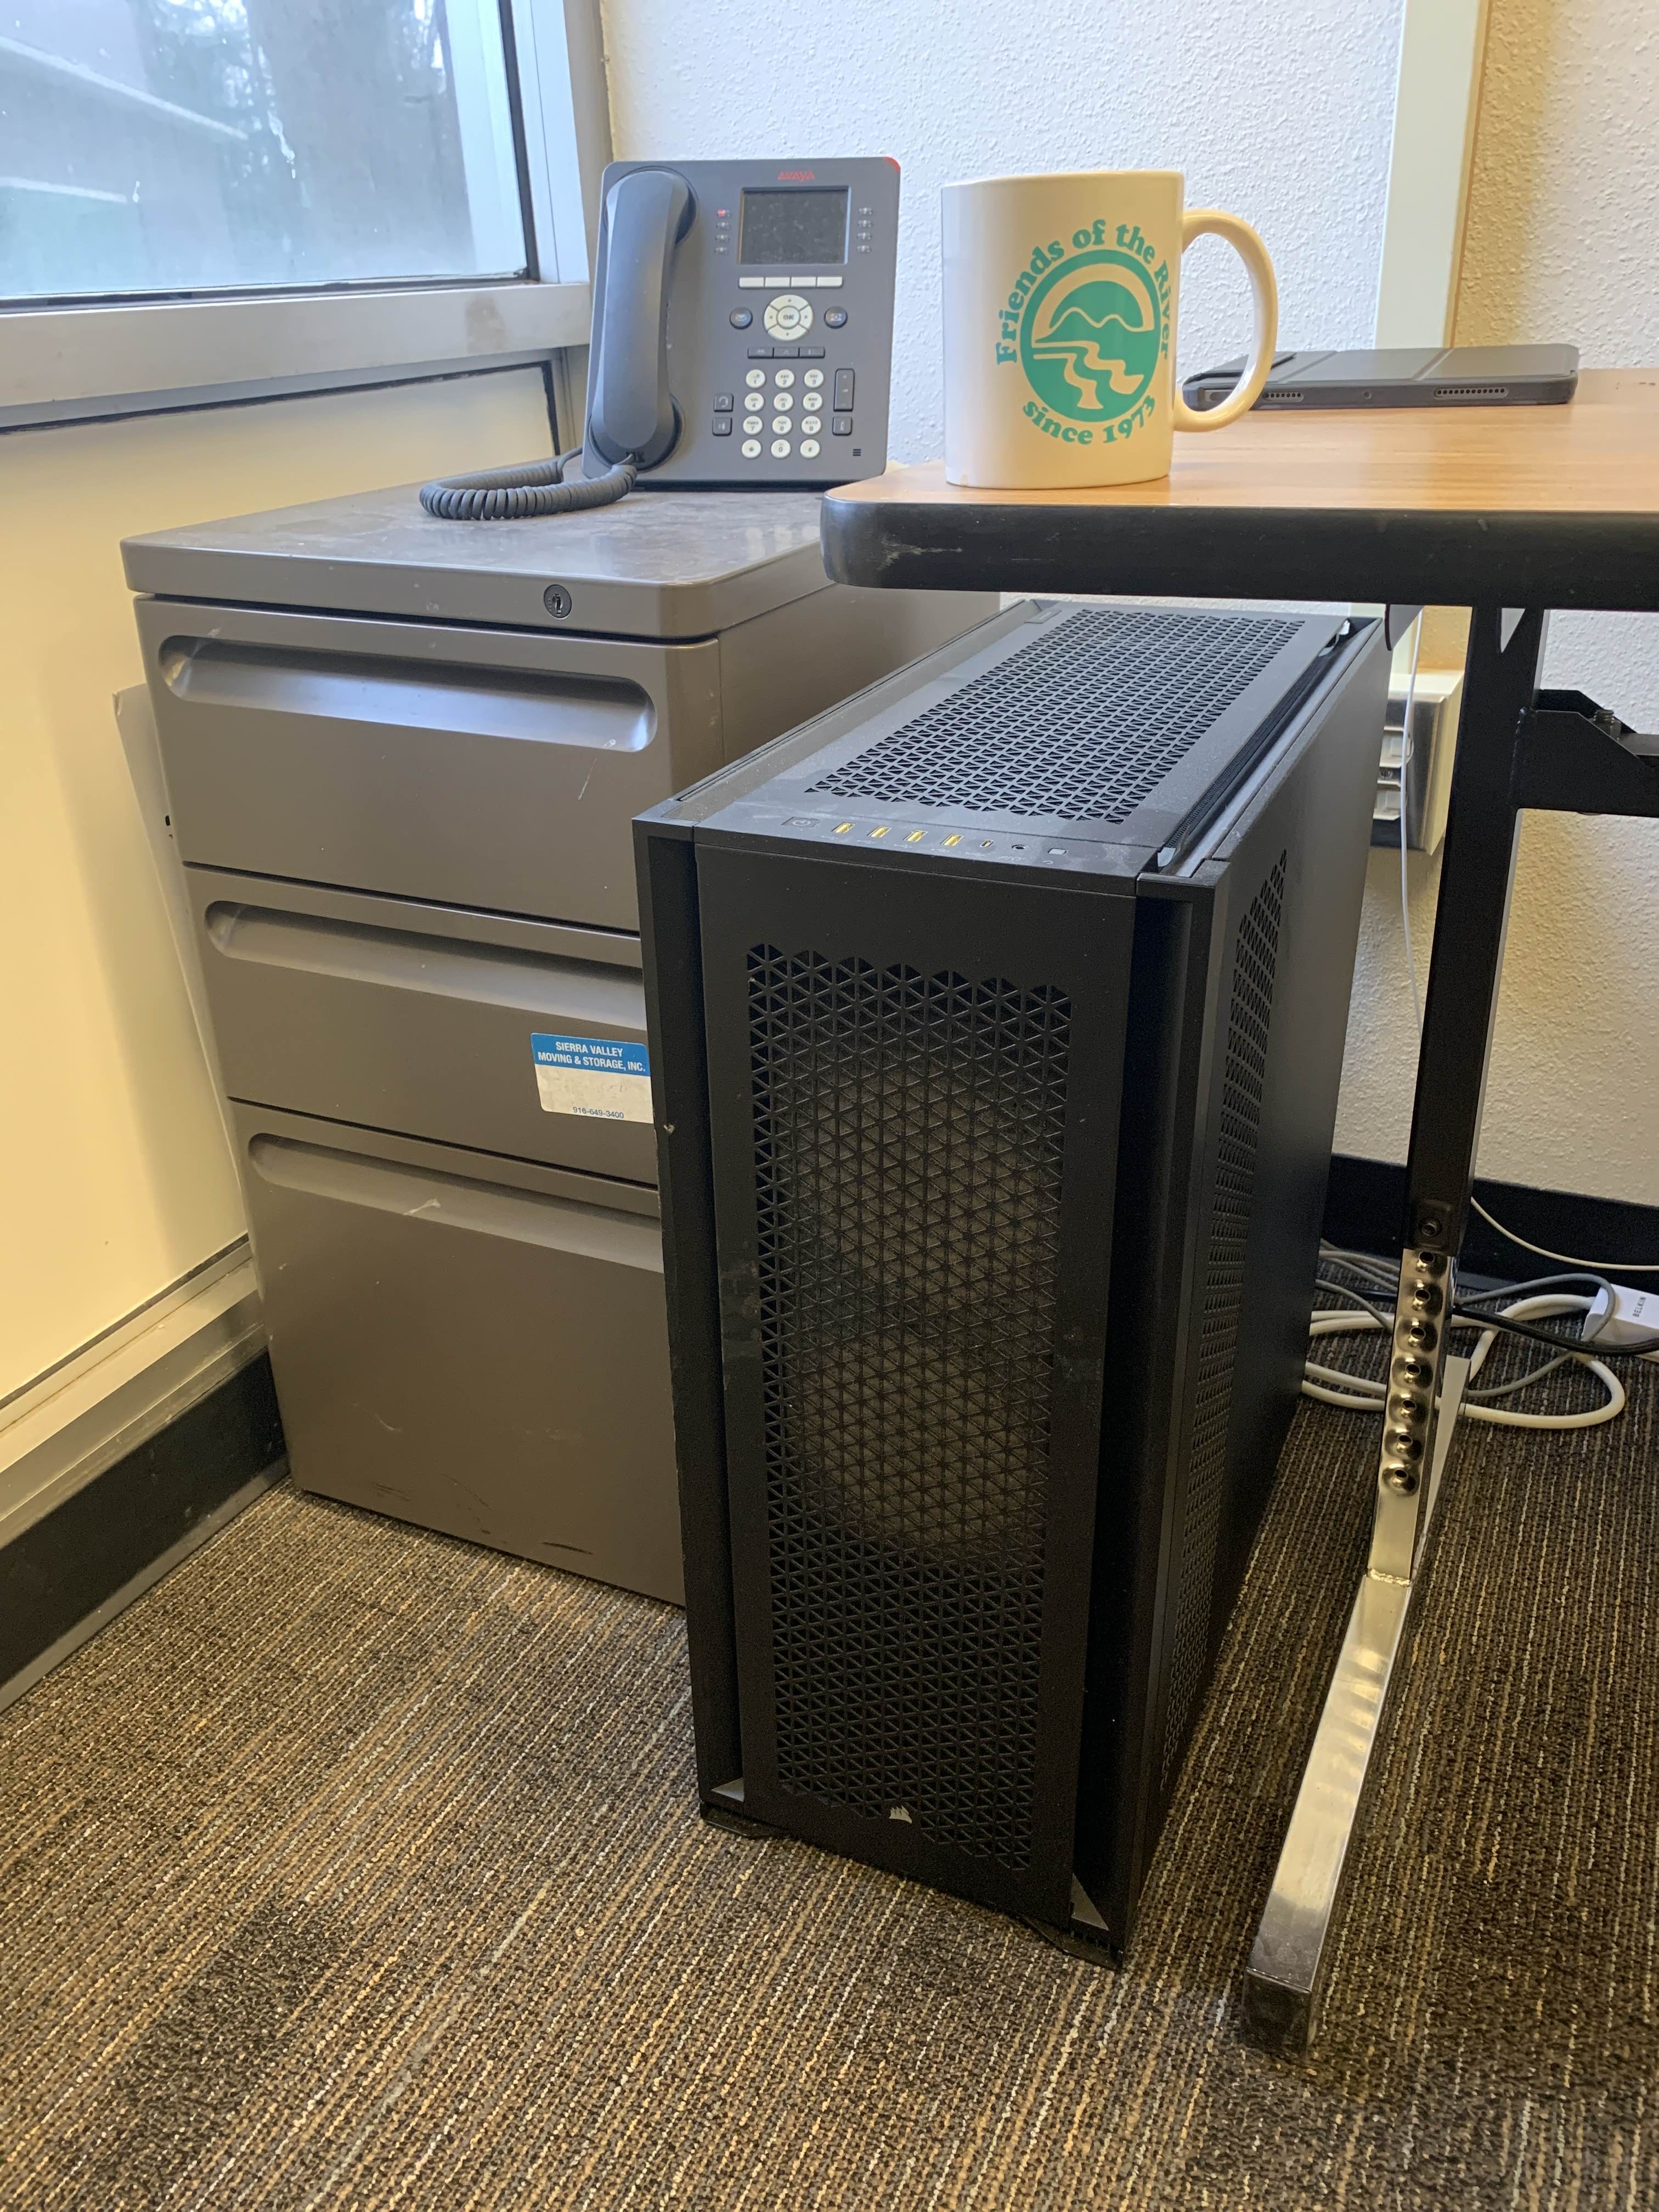
\includegraphics[width=0.5\textwidth]{server}
    \caption{A simple server under a desk works just fine for teaching.}
    \label{fig:server}
\end{figure}

The major advantages of the personal physical server are cost and simplicity.
Regarding cost, we've found it easier to fund a one time purchase of a few thousand dollars compared to finding a sponsor who will commit to the ongoing variable subscription fees of the cloud services, even if the total cost would be lower for the cloud subscription.
It's simple because you can set it up one time, and then use the same machine for several years.
We didn't need any specialized knowledge beyond the basics.
We completely own and administrator the machine, so we can install whatever we want, whenever we want.
It's relatively easy and direct to automate certain grading tasks, for example, an instructor can use administrative privileges to look at \texttt{history} to see every command a student typed during a quiz.

The disadvantage of a single physical machine is that if there is a problem, then it affects the entire class, and we are our own support.
Students have made mistakes and filled up all the disk space, and we needed to diagnose and fix the issue on our own.
Pedagogically, this mistake followed by the unusable server highlights the importance of not creating unnecessary copies when working with large amounts of data, and it makes students more aware of how much data they're saving.
The fix is straightforward: just delete the big files that the students accidentally made copies of.
A more proactive solution to this common problem is to impose a quota on disk usage.
We're taking a risk that the server could fail in a more serious way, but it's a calculated risk.

%when the students make a mistake and fill up all the disk space, it does not affect anyone or anything outside of the class.
%If we spill coffee on the machine, or it fails 
%Nothing else essential is running on the machine, so 
%If something goes wrong, I'm the only one who's going to fix it.
%We don't have to worry about any creating and maintaining cloud images.

The server doesn't need to be particularly powerful or expensive.
For a class of 15 students, we found that a single 32 core CPU, a GPU, and 128 GB of memory was just sufficient for students to experience the class assignments in the way we intended.
This machine cost around \$3,000 when purchased in 2022.
We always recommend that students do their homework well before the due date, because if a handful of users are simultaneously trying to use parallel jobs with all available CPU cores, then they won't see the speedup they are expecting.
In practice it happened occasionaly that students who waited until the last hour to do an assignment didn't get to see their final result, but they weren't surprised, because we had warned them many times and they knew to expect this.
We've used a 16 core CPU machine in previous semesters, and found that it was not sufficient for 15 students.
With more students, we believe that students would feel crowded on the server.

One technical detail to be aware of is that you must provide remote access so that others can log on to the machine.
Campus IT handled this by providing a DNS hostname.
Our students need to be either on campus or at home on the campus VPN (Virtual Private Network), and they can login via ssh, for example: \texttt{ssh fitzgerald@nsm-stats.csus.edu}.
We recommend against setting up a physical server at your home, because providing reliable remote access could be tough depending on your internet provider, and there's no reason you should pay for the electricity instead of campus.

The physical server feels out of date, and lacks the cachet of being `the cloud'.
Despite that, it provides a legitimate and simple way to get students using a remote server.
From a student's perspective, there's no difference between \texttt{ssh} to this machine, or to a virtual machine that you own that's running on the cloud.

\subsection{Cloud}

The cloud offers the most flexibility of all the server options.
Indeed, all the different ways one could potentially use and teach cloud services can be overwhelming.
In Stat 129, students process data by logging into a virtual machine (VM), a logical rather than a physical computer.
We've experimented with two ways of providing students with cloud access: administrative accounts on the cloud, or local user accounts on a VM.
We've used both of these options, and they both have a place, depending on the goals of the class.

Administrative cloud accounts provide students with a richer cloud experience, as they create their own virtual machines which they have complete control over.
They are the administrators to these machines with \texttt{sudo} access, so they can do anything they wish, and any mistakes they make won't affect anyone else.
Load balancing has the potential to work better in this scenario, as students can create machines that are as large as they like, and delete them when they are done.
This would be a good option if the course is designed to teach them more about infrastructure, for example, how to implement a full stack web application.
This rich experience does come with some additional complexity and responsibility, for example, students need to load and save their results as they create and delete machines.

Local user accounts on a single VM allow students to focus more on the data analysis rather than the cloud ideas and infrastructure.
In this scenario the instructor creates a VM that's large enough to accommodate all of the students simultaneously, and students access through SSH or a web interface.
The downside here is that you need to pay for a large enough machine all the time, or else manually load balance by switching to smaller or larger machines as the demand changes.
%If we were goint

Note that you can combine the simpler single VM accounts together with the richer administrative accounts.
For example, we have started the semester with a single VM large enough for the class, which students all students log in to and use for simple assignments and in class activities, and then later in the semester students progress to setting up their own VM's.
Now we turn our attention to cloud provider options.


% TODO: mention RStudio somewhere

\subsubsection{Public Cloud}

We have had an excellent experience teaching Stat 129 using the NSF funded cloud provider, Jetstream2 \cite{hancock2021jetstream2}.
In this model, the instructor applies for an allocation, the reviewers award a certain number of compute hours, and the instructor sets up the accounts on the machines.
We applied, were approved, and had everything set up in less than a week.
In fact, the reviewer awarded TODO explain SU's

The Jetstream2 website\footnote{\url{https://jetstream-cloud.org/index.html}} states:
\begin{quote}
Jetstream2 makes cutting-edge high-performance computing and software easy to use for research regardless of your project’s scale, even if you have limited experience with supercomputing systems.

Cloud-based and on-demand, the Jetstream2 environment also includes discipline-specific apps. You can even create virtual machines that look and feel like your lab workstation or home machine—but with thousands of times the computing power.
\end{quote}

The benefits of Jetstream2 are the free cost for students, the simplicity compared to commercial cloud providers, and the ability to connect seamlessly to large data sets.
Thanks to NSF funding, our students, many of whom are low income, received accounts without needing to provide a credit card.
The user interface and options are much simpler than commercial cloud providers, and they cater directly to the academic wishing to analyze large data sets through Manila Filesystems as a service.
Figure~\ref{fig:jetstream} shows an example of the clean web user interface to create a new instance of a VM.
We followed the Jetstream2 documentation and mounted a 1 TB Manila file share to the VMs, which allowed students to simultaneously access and analyze shared data as if it was local to their machine \cite{manila}.
In our experience, Jetstream2 has lived up to its claims of making cloud computing easy and accessible.

\begin{figure}[h]
    \centering
    \includegraphics[width=0.5\textwidth]{jetstream}
    \caption{The Jetstream2 user interface is far simpler and easier to teach compared to commercial cloud providers.}
    \label{fig:jetstream}
\end{figure}

The disadvantages of Jetstream2 for teaching college classes are the security model, the lack of safeguards, and the annual renewals.
Jetstream2 prioritizes the needs of individual researchers and small research groups, and they support this primary use case very well.
Jetstream2 is not designed primarily for teaching a semester long undergraduate class with 30 students.
When the reviewers award the instructor an allocation, every user gets complete access to every part of the account on the allocation.
If you give students user accounts so that they can have the administrative experience of creating their own VM's, then they will have administrative access to everything the instructor creates, and to every other student's machine.
There are no limits on how much compute a particular user can use, so it's possible for one user to use up all the credits for the allocation.
In other words, the only thing that's stopping them from doing something bad is their own awareness and respect for others.
We mostly got around these issues by setting very clear expectations for behavior, with the understanding that this whole idea is based on trust.
Even so, a student unintentionally left a large machine running for several weeks.
We weren't monitoring as diligently as we should have, and this used up a significant portion of our 100,000 service units, but we still had plenty to get through the course.
Finally, our allocation on Jetstream2 required annual renewal, which makes us hesitate to rely on it as a long term solution for teaching Stat 129.
We expect the reviewers would renew every year if there is funding available, but there are no guarantees.
This isn't an issue if someone is paying for commercial cloud services.


\subsubsection{Commercial Cloud}
\label{sec:comcloud}

Several companies offer commercial cloud services.
We focused mainly on Amazon Web Services (AWS), the biggest and most popular vendor, to provide our students with marketable experience that they can then put on their resume.
Our favorite feature of AWS is the direct access to Amazon's high quality open data sets through the \texttt{aws s3} command line tools.
From an instructor's perspective, this eliminates the step of downloading the data and making it available to students.

A sustainable funding model for teaching a class like Stat 129 is to make students pay for commercial cloud services, and this doesn't need to be expensive.
In Spring 2022, we found that students on AWS can get a rich data processing experience for \$20 or less in one semester, which is less than a low cost textbook for a single course.
These are commercial services, so a student must have a credit card and be prepared to pay for any compute time and storage that they use.
However, if they make a mistake, say using a powerful VM and forgetting to shut it off, then they can easily run up an expensive and unexpected bill that can be tough for a college student to cover.
In the past, AWS offered an educational program with free credits for students, which didn't even require a credit card.
We used this program, but they discontinued it, which left us looking for other free options.

Complexity and vendor specificity are problems when teaching with cloud services.
Amazon's EC2 (cloud compute server) allows students to create their own VM's, and it ``provides a wide selection of over 750 instance types optimized to fit different use cases.''\cite{aws-ec2}
There are also hundreds of different services and many world regions to choose from.
This is an overwhelming amount of choice for a student or even an instructor, and the available options change regularly.
Furthermore, the services often have company specific names, which makes it difficult for an instructor to understand what they are.
Indeed, the main purpose of the `AWS Cloud Practitioner' qualification seems to be to understand all of these proprietary names and services.
As faculty at a public institution, our goal is to focus on the overarching concepts and portable technologies that a student can take and apply anywhere, regardless of the specific vendor.

While we feel that the commercial cloud services aren't currently the best choice for teaching Stat 129 at CSU Sacramento, they might be the best choice for you.
If you already have experience with a particular cloud provider, or you wish to build that experience from the ground up, then this is an opportunity. 
If your institution has some connection with a cloud provider, then it may be mutually beneficial to leverage those connections.
For example, the company may provide cloud services for free in exchange for the access to recruit graduates into that company.
If the goal of your course is to focus more on a specific technology such as R, Python, or SQL then you should consider popular vendors such as Posit Cloud (formerly RStudio), Anaconda Cloud, or Snowflake.
These vendors use commercial cloud services as a foundation, abstract away many of the complicated details of server administration, and provide a familiar web based user interface.

None of the available cloud services that we've explored or mentioned are ideal for teaching Stat 129.
We conclude by describing what emph{would} be ideal, based on our experience.

\section{Moving Forward}

If it was easier to set up and run a server for teaching undergraduate data analysis classes like Stat 129, then we believe that more instructors would be interested in teaching these courses.
For a lone instructor with a heavy teaching load and no support, the barriers to entry are significant.
We would welcome a shared solution, cloud or otherwise, that provides this capability publicly to instructors simultaneously teaching similar courses at other institutions.
It should have the following features:
\begin{enumerate}
\item \textbf{100 GB shared data storage} It should be easy for an entire class to simultaneously read and share the same large data sets.
    1 TB of storage would be better.
\item \textbf{data science tools} Students should be able to use common data science programming technogies such as R, Python, and some form of SQL.
    One way to provide this is to give the instructor administrative privileges to install software.
    Web based clients using tools such as Jupyter Notebooks certainly broaden the appeal and potential users of the server, but they are not strictly necessary.
\item \textbf{free or low cost} Free for students is ideal, of course.
    If free is not possible, then the cost over the semester should not exceed that of a reasonably priced textbook.
\item \textbf{instructor support}
    Instructors without a background in systems administration should be able to teach on the server, and receive some level of technical and community support.
    This is perhaps the hardest requirement, because the best way to provide dedicated support is through paid staff.
\item \textbf{long term sustainability} 
    If instructors and institutions are going to invest in creating courses that rely on a server, then they need to have some assurance that the server will continue to exist.
    A 1 year pilot program might be a useful start, but it's much more compelling to have a guarantee that a server will be available for the next 5 years.
\item \textbf{minimal specificity}
    It's ideal if students in a one semester data science class don't need to learn concepts specific to one particular system or vendor, as discussed in Sections~\ref{sec:server} and~\ref{sec:comcloud}.
\item \textbf{novice user safeguards} It should not be possible for one student to delete or damage course infrastructure, either accidentally or on purpose.
    Standard Linux user accounts without administrative privileges work fine.
\item \textbf{parallel capability}
    The parallel processing capabilities of the server should exceed those of a common laptop to provide a compelling reason to actually use the server.
    In practice, if there are 10 CPU's available, then students can experience an order of magnitude speedup compared to a serial program, and this is enough to motivate the techniques in Stat 129.
    An abundance of compute power is definitely not necessary if instructors follow the advice in Section~\ref{sec:data}.
\item \textbf{shell access} Students should be able to interact with their computer using bash so that they can use data processing pipelines, scripts, and version control.
\end{enumerate}

The above instructor level requirements imply other requirements at the system level, and these require serious thought.
For example, if a shared solution is going to simultaneously support 20 instructors teaching 400 students, then load balancing is a real concern.
We leave the system level requirements to the professionals.

Fostering a culture of support, mentorship, and growth for teaching unfamiliar but valuable data analysis technologies is more important than the logistics of setting up a server.
Academia as a whole, and mathematics and statistics department in particular, need to value programming skills and find ways to support instructors who may be teaching new and unfamiliar topics.

Large data sets are here to stay, and we serve our our statistics students well by teaching them how to actually work with large data.
It's quite uncommon to see a course designed around the student experience on a server, particularly in a mathematics and statistics department.
We hope that in the future compute servers become to a statistics program somewhat like physical laboratory space is to a chemistry program: a necessity.

%We hope to see more courses like Stat 129 are offered in the future.

\bibliographystyle{plain}
\bibliography{references}

\end{document}
